\documentclass[a4paper, 12pt]{article}

\usepackage[cm-default]{fontspec}
\usepackage{listings}
\usepackage{graphicx}
\usepackage{adjustbox}
\usepackage{array}
\usepackage{tabularx}
\usepackage{booktabs}
\usepackage{indentfirst}
\usepackage{textcomp}
\usepackage{enumitem}
\usepackage{lastpage}
\usepackage{fancyhdr}
\usepackage[top = 2.8cm, bottom = 2cm, left = 2cm, right = 2cm]{geometry}
\usepackage[BoldFont,SlantFont,CJKchecksingle]{xeCJK}

\newfontfamily{\lstfont}[Scale=.75]{Consolas}
\newfontfamily{\inlinecode}[Scale=.9]{Consolas}
\pagestyle{fancy}
\fancyhf{}

\rfoot{第 \thepage \hspace{1pt} 页,共 \pageref{LastPage} 页}
\XeTeXlinebreaklocale "zh"

\graphicspath{ {imgs/} }
\newfontfamily\codeFont[]{Consolas}
\newfontfamily\commentFont[]{黑体}
\newfontfamily\heiti[]{黑体}
\setCJKmainfont[BoldFont=SimHei]{SimSun}
\parindent 2em

\lstdefinelanguage{HTTP}{
  keywords={?, &},
  morecomment=[l]{//},
  morecomment=[s]{/*}{*/},
  morestring=[b]',
  morestring=[b]",
  ndkeywords={POST, GET, PUT, DELETE, MERGE, FETCH},
  basicstyle=\lstfont,
  keywordstyle=\lstfont\textbf,
  ndkeywordstyle=\lstfont\textbf,
  identifierstyle=\color{black},
  commentstyle=\commentFont,
  stringstyle=\lstfont,
  sensitive=true,
  extendedchars=false
}
\lstdefinelanguage{javascript}{
  keywords={let, var, function, return, for, do, while, switch, case, default, module, export, yield, const, in, from, import, if, else, this},
  morecomment=[l]{//},
  morecomment=[s]{/*}{*/},
  morestring=[b]',
  morestring=[b]",
  ndkeywords={Array, Promise, String, Object, ArrayBuffer},
  basicstyle=\lstfont,
  keywordstyle=\lstfont\textbf,
  ndkeywordstyle=\lstfont\textbf,
  identifierstyle=\color{black},
  commentstyle=\lstfont\textbf,
  stringstyle=\lstfont,
  sensitive=true,
  breaklines=true,
  breakatwhitespace=false,
  extendedchars=false
}
\lstdefinelanguage{json}{
    showstringspaces=false,
    literate=
     *{0}{{{\color{numb}0}}}{1}
      {1}{{{\color{numb}1}}}{1}
      {2}{{{\color{numb}2}}}{1}
      {3}{{{\color{numb}3}}}{1}
      {4}{{{\color{numb}4}}}{1}
      {5}{{{\color{numb}5}}}{1}
      {6}{{{\color{numb}6}}}{1}
      {7}{{{\color{numb}7}}}{1}
      {8}{{{\color{numb}8}}}{1}
      {9}{{{\color{numb}9}}}{1}
      {:}{{{\color{punct}{:}}}}{1}
      {,}{{{\color{punct}{,}}}}{1}
      {\{}{{{\color{delim}{\{}}}}{1}
      {\}}{{{\color{delim}{\}}}}}{1}
      {[}{{{\color{delim}{[}}}}{1}
      {]}{{{\color{delim}{]}}}}{1},
}


\begin{document}
\begin{titlepage}

\begin{center}
	\marginbox{0cm 2cm 0cm 3cm}{\includegraphics[width=2.67cm, height=2.67cm]{logo}}
	\marginbox{1.6cm 2cm 0cm 3cm}{\includegraphics[height=2.67cm]{logo2}}
	\marginbox{0cm 1cm 0cm 0cm}{\fontsize{42pt}{0}\selectfont 大型数据库设计与应用}	
	\marginbox{0cm 2cm 0cm 0cm}{\fontsize{32pt}{0}\selectfont 实 \ 习 \ 报 \ 告}	
\end{center}
{\fontsize{14pt}{0}\selectfont
	\marginbox{1.5cm 0cm 0cm 0cm}{设计题目:{\underline{\hspace{1.85cm} 知识产权管理系统大型数据库设计 \hspace{1.85cm}}}} \\ \\ \\
	\marginbox{1.5cm 0cm 0cm 0cm}{学生姓名:{\underline{\hspace{.3cm} 张宇泽 \hspace{.3cm}}}  班级:{\underline{\hspace{.2cm} 软件141 \hspace{.2cm}}}  学号:{\underline{\hspace{.46cm} 14477135 \hspace{.46cm}}}} \\ \\ \\ 
	\marginbox{1.5cm 0cm 0cm 0cm}{学院(系):{\underline{\hspace{.5cm} 信息数理学院 \hspace{.5cm}}}  指导老师:{\underline{\hspace{.85cm} 石林,傅东 \hspace{.85cm}}}} \\ \\ \\ 
	\marginbox{1.5cm 0cm 0cm 0cm}{设计日期:{\underline{\hspace{1.10cm}  2016年12月26日 - 2017年01月04日 \hspace{1.10cm}}}} \\ \\ \\
	\marginbox{1.5cm 0cm 0cm 0cm}{成  绩:{\underline{\hspace{11.4cm}}}} \\ \\ \\
	\marginbox{1.5cm 0cm 0cm 0cm}{评阅日期:{\underline{\hspace{11.4cm}}}}
}
\end{titlepage}

\setmainfont{Times New Roman}

\begin{center}
  \fontsize{18pt}{0}\selectfont{知识产权管理系统大型数据库设计任务书} \\
\end{center}

{\setlength\extrarowheight{6pt}
	\begin{tabular}{|c|l|}
		\hline
		\multicolumn{2}{|l|}{ 一、设计题目 } \\
		\multicolumn{2}{|l|}{ 知识产权管理系统大型数据库设计 } \\
		\hline
		\multicolumn{2}{|l|}{ 二、设计内容及目标 } \\
		\multicolumn{2}{|l|}{ 1)查相关资料,设计系统的实施方案;} \\
		\multicolumn{2}{|l|}{ 2)进行数据库设计,绘制 E-R 图;} \\
		\multicolumn{2}{|l|}{ 3)建立数据库,开始编码;} \\
		\multicolumn{2}{|l|}{ 设计目标:} \\
		\multicolumn{2}{|l|}{ 1)系统主要功能模块包括:字典管理,执法人员管理和新闻政策;其中,字典管} \\
		\multicolumn{2}{|l|}{ 理和执法人员管理均为对字典和执法人员的增删改;新闻政策管理可以发布、启} \\
		\multicolumn{2}{|l|}{ 用、禁用、预览、查询新闻和策略内容。} \\
		\multicolumn{2}{|l|}{ 2)对用户实现权限分级管理,并做好防提权、防注入。} \\
		\multicolumn{2}{|l|}{ 3)界面友好、软件运行稳定运行} \\
		\hline
		\multicolumn{2}{|l|}{ 三、进度安排 } \\
		\hline
		日期 				& \multicolumn{1}{c|}{工 \ 作 \ 内 \ 容} \\
		\hline
		12月26日 			& 任务安排,了解需求,分析实体 \\
		\hline
		12月27日 			& 设计数据库,使用SQL语句建库 \\
		\hline
		12月28日~01月4日	& 设计程序,开始编码 \\
		\hline
		01月5日	& 完成实验报告 \\
		\hline
		\multicolumn{2}{|l|}{ 四、设计日期 } \\
		\hline
		\multicolumn{2}{|l|}{ 2016年12月26日 - 2017年01月04日 } \\
		\hline
	\end{tabular}
}
	\thispagestyle{empty}
	\clearpage
	\setcounter{page}{1}
	\setlength{\parskip}{-0.1em}

	\section{\large\textbf 前言}
	\subsection{\normalfont 系统概述}
	
	随着企业专利、商标、版权、域名等的日积月累,企业知识产权管理工作,正在变得越来越重要。
	要有效的掌控自己的知识产权,仅靠手工操作,将是一件繁琐而风险极高的工作。
	因此,设计一个跨平台的、网络化的知识产权管理系统十分必要。

	\subsection{\normalfont 主要功能}

	受时间等因素限制,此次课程设计仅完成完整系统中的三个功能点,分别是:字典管理、执法人员管理和新闻
	政策管理。若登陆用户拥有足够的权限时,可以对这三个功能点中的数据进行添加、查询、编辑和删除操作。
	后端接口支持权限的分级管理,可以有效的保证数据安全和稳定。

	\subsection{\normalfont\large\normalfont 使用方法}

	为了降低使用难度,方便用户接入,本次课设采用 B/S 架构,用户仅仅需要一个支持 JavaScript 的浏览器
	即可正常使用所有功能。在网页中,数据将以表格的形式展示,单击其中的数据行即可对数据进行编辑或删除。
	
	\section{\large\textbf 需求描述}
	
	\subsection{\normalfont 字典管理}
	点击字典管理,可对字典数据进行新增和修改操作。

	\subsection{\normalfont 执法人员管理}
	点击执法人员管理,可对执法人员信息进行新增和修改操作。

	\subsection{\normalfont 新闻政策}
	点击新闻政策菜单,显示区域显示已发布的新闻政策,包括新闻标题,新闻类型,文件类型,新闻状态等信息。
	同时显示区域上方可对新闻政策信息进行过滤查询,并有发布新闻,启用或禁用某条新闻,修改新闻和预览新闻
	等按钮。

	\begin{enumerate} 
	{\setlength{\parskip}{-0.3em}
		\item 新闻查询通过新闻标题对新闻进行过滤,筛选出符合条件的新闻。
		\item 点击发布新闻,可在线填写新闻标题,选择文件类型和新闻分类,并可在线编辑要发布的新闻或政策的内容。
		\item 点击启用/禁用,可改变单条新闻的状态,启用或禁用该条新闻。
		\item 选中新闻后,点击修改新闻,可对新闻标题,新闻类型和新闻内容进行更改。
		\item 点击新闻预览,可预览选中的新闻。
	}
	\end{enumerate}

	\section{\Large\textbf 数据库应用}

	\subsection{\normalfont 实体关系分析}

	根据需求,可以分析得到执法人员、新闻政策和字典的关系:执法人员创建并管理新闻政策,同时执法人员和新闻政策的属
	性信息中的关键字通过类似 Map 数据结构,映射到字典表中的具体内容。由此可以得到实体关系图(E-R 图)如下图(1)
	所示:

	\begin{center}
		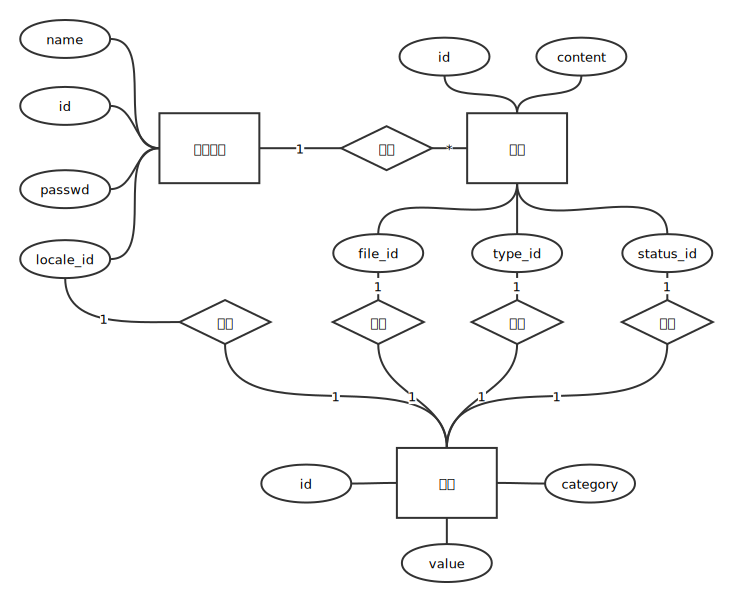
\includegraphics[width=12cm]{ER.pdf} \\
		\scriptsize 图(1)实体关系图
	\end{center}

	\subsection{\normalfont 数据库软件与设计}

	服务端使用 MariaDB 进行开发,MariaDB数据库管理系统是MySQL的一个分支,主要由开源社区在维护,采用GPL授权
	许可。 根据需求说明,该程序至少需要三张数据表:

	\begin{enumerate} 
	{\setlength{\parskip}{-0.3em}
		\item 字典表
		\item 执法人员表
		\item 新闻政策表
	}
	\end{enumerate}

	同时,为了满足上述的映射关系,需要使用外键来约束相应的表项另外,为了完成用户的登陆和验证以及权限控制,我
	们还需要一张用户,一张登陆状态表。设计分别如下:

	\subsubsection{\normalfont 字典表}

	\begin{tabular}{l|l|l|l}
		\toprule
		\multicolumn{1}{c|}{字段名}	& \multicolumn{1}{c|}{字段类型}	& \multicolumn{1}{c|}{默认值}	& \multicolumn{1}{c}{说明} \\
		\midrule
		dict\_id					& INTEGER 						& 								& 字典 ID \\
		\midrule
		dict\_category				& VARCHAR(100) 					& 								& 字典类型 \\
		\midrule
		dict\_value					& VARCHAR(100)					& 								& 字典内容 \\
		\bottomrule
	\end{tabular} \\

	其中,dict\_category 为常量,值如下:

	{\setlist[enumerate,1]{start=0}
		\begin{enumerate} 
		{\setlength{\parskip}{-0.3em}
			\item (NEWS\_TYPE)   $\,\to\,$ 新闻类型字典
			\item (NEWS\_STATUS) $\,\to\,$ 新闻状态字典
			\item (FILE\_TYPE)   $\,\to\,$ 文件类型字典
			\item (LOCALE)       $\,\to\,$ 地区字典
		}
		\end{enumerate}
	}

	\subsubsection{\normalfont 执法人员}

	\begin{tabular}{l|l|l|l}
		\toprule
		\multicolumn{1}{c|}{字段名}	& \multicolumn{1}{c|}{字段类型}	& \multicolumn{1}{c|}{默认值}	& \multicolumn{1}{c}{说明} \\
		\midrule
		officer\_id					& INTEGER 						& 								& 执法人员 ID \\
		\midrule
		officer\_name				& VARCHAR(50)					& 								& 执法人员名字 \\
		\midrule
		officer\_geder				& VARCHAR(10)					& 								& 执法人员性别 \\
		\midrule
		officer\_major				& VARCHAR(50)					& 								& 执法人员专业 \\
		\midrule
		officer\_job				& VARCHAR(50)					& 								& 执法人员职务 \\
		\midrule
		officer\_license\_id		& VARCHAR(50)					& 								& 执法人员许可编号 \\
		\midrule
		officer\_locale\_id			& INTEGER 						& 								& 执法人员工作地区,外键 \\
		\midrule
		user\_id					& INTEGER 						& 								& 执法人员用户 ID(用于登录) \\
		\bottomrule
	\end{tabular} \\

	\subsubsection{\normalfont 新闻政策}

	\begin{tabular}{l|l|l|l}
		\toprule
		\multicolumn{1}{c|}{字段名}	& \multicolumn{1}{c|}{字段类型}	& \multicolumn{1}{c|}{默认值}	& \multicolumn{1}{c}{说明} \\
		\midrule
		news\_policy\_id			& INTEGER 						& 								& 新闻政策 ID \\
		\midrule
		news\_title					& VARCHAR(250)					& 								& 新闻名称 \\
		\midrule
		news\_content				& TEXT							& 								& 新闻内容 \\
		\midrule
		news\_date					& DATE							& 								& 新闻日期 \\
		\midrule
		news\_type\_id				& INTEGER						& 								& 新闻类型 ID,外键 \\
		\midrule
		new\_status\_id				& INTEGER						& 								& 新闻状态 ID,外键 \\
		\midrule
		file\_type\_id				& INTEGER 						& 								& 文件类型 ID,外键 \\
		\midrule
		publish\_officer\_id		& INTEGER 						& 								& 发布的执法人员 ID,外键 \\
		\bottomrule
	\end{tabular} \\

	\subsubsection{\normalfont 用户表}

	\begin{tabular}{l|l|l|l}
		\toprule
		\multicolumn{1}{c|}{字段名}	& \multicolumn{1}{c|}{字段类型}	& \multicolumn{1}{c|}{默认值}	& \multicolumn{1}{c}{说明} \\
		\midrule
		user\_id						& INTEGER						& 								& 用户 ID \\
		\midrule
		username					& VARCHAR(100)					& 								& 登录名 \\
		\midrule
		password					& VARCHAR(100) 					& 								& 登录密码 \\
		\midrule
		role						& INTEGER						& 								& 用户角色 \\
		\bottomrule
	\end{tabular} \\

	其中,role 为常量,值如下:

	{\setlist[enumerate,1]{start=0}
		\begin{enumerate} 
		{\setlength{\parskip}{-0.3em}
			\item (ADMINISTRATOR)   $\,\to\,$ 最高管理员
			\item (OFFICER) $\,\to\,$ 执法人员
			\item (COMMON)   $\,\to\,$ 普通用户
			\item (DELETED)       $\,\to\,$ 已删除账户
		}
		\end{enumerate}
	}

	\subsubsection{\normalfont 登录状态表}

	\begin{tabular}{l|l|l|l}
		\toprule
		\multicolumn{1}{c|}{字段名}	& \multicolumn{1}{c|}{字段类型}	& \multicolumn{1}{c|}{默认值}	& \multicolumn{1}{c}{说明} \\
		\midrule
		access\_token				& VARCHAR(100)					& 								& 访问密钥 \\
		\midrule
		user\_id					& VARCHAR(100) 					& 								& 密钥拥有者 ID \\
		\bottomrule
	\end{tabular} \\


	\section{\large\textbf 程序设计}
	\subsection{\normalfont 概述}

	为了获得性能上的提升,程序运行在 Linux 平台下,使用异步操作,事件驱动的 Node.js 作为开发语言。 由
	于 MariaDB 在设计上是与 MySQL 完全兼容的,我们可以直接借助 MySQL 的相关连接组件来完成数据库和程序
	语言的交互。 网页程序设计为单页应用,主要代码在浏览器中以 JavaScript 的形式运行,而数据交互和用户
	验证则依赖于符合 RESTful 原则 的后端 API 组成。与 SOAP 和 XML-RPC 相比,REST 更加简洁,并易于理
	解和使用。

	\subsection{\normalfont API 设计}

	参考 RESTful 要求,我们将三张表的操作设计为对三个 URL 的操作,并使用不同的{\inlinecode HTTP Method}来指明操作的内容,例如:

	\begin{lstlisting}[language=HTTP, basicstyle=\small\lstfont, showstringspaces=false]
	GET /api/v1/user
	\end{lstlisting}

	即为获取所有的用户信息,结果以{\inlinecode JSON}的形式回复。\\

	若需要指定查询的满足条件,可以在{\inlinecode URL}中添加查询,例如:

	\begin{lstlisting}[language=HTTP, basicstyle=\small\lstfont, showstringspaces=false]
	GET /api/v1/user?role=ADMINISTRATOR
	\end{lstlisting}

	即为获取所有类型为系统管理员的用户信息。\\

	当需要对部分内容进行更新操作时,使用{\inlinecode HTTP POST}方法来完成,例如:

	\begin{lstlisting}[language=HTTP, basicstyle=\small\lstfont, showstringspaces=false]
	POST /api/v1/dict?value=International%20News&id=1&type=NEWS_TYPE
	\end{lstlisting}

	即为将 ID 为 1 的字典项的值设置为 International News,将其类型设置为{\inlinecode NEWS\_TYPE}。\\

	当需要创建信息时,使用{\inlinecode HTTP PUT}方法来完成,例如:
	
	\begin{lstlisting}[language=HTTP, basicstyle=\small\lstfont, showstringspaces=false]
	PUT /api/v1/dict?value=International%20News&type=NEWS_TYPE
	\end{lstlisting}

	即可创建一个字典项。与{\inlinecode HTTP POST}不同,创建不需要指定 ID。

	\subsection{\normalfont 用户验证设计}

	为了保证信息安全性,同时实现用户权限的分级控制,以上所有 API 的接口都需要进行身份验证。后端 API 在
	接受请求之后将会确认{\inlinecode token}这个查询是否存在,若存在,则在{\inlinecode token}表中查询
	是否是合法的访问密钥,并以此确定用户身份。若查询结果 为无效{\inlinecode token},或
	{\inlinecode token}未定义,则将返回包含 Unauthorized Access 信息的{\inlinecode JSON}。

	用户首先要使用用户名和密码进行登陆,但是不能将用户名和密码直接保存在客户端浏览器,所以需要设计一个
	验证 Portal,在 这里完成用户名和密码的组合验证,完成之后,返回一个有效的 Access token。所有后续的
	访问都需要使用此{\inlinecode token}的合法性。 例如:

	\begin{lstlisting}[language=HTTP, basicstyle=\small\lstfont, showstringspaces=false]
	GET /api/v1/portal?username=foo&password=bar
	\end{lstlisting}

	若此用户名和密码的组合有效,则返回:

	\begin{lstlisting}[language=json, basicstyle=\small\lstfont, showstringspaces=false]
	{
	  "status": "ok",
	  "token": "someVeryLongAndRandomString"
	}
	\end{lstlisting}

	相反,则:

	\begin{lstlisting}[language=json, basicstyle=\small\lstfont, showstringspaces=false]
	{
	  "status": "err",
	  "msg": "unauthorized access"
	}
	\end{lstlisting}

	后续请求需要使用这个 token 来表面用户的身份,例如:

	\begin{lstlisting}[language=HTTP, basicstyle=\small\lstfont, showstringspaces=false]
	GET /api/v1/user?token=someVeryLongAndRandomString
	\end{lstlisting}

	即可通过验证并取得信息。否则返回 Unauthorized Access。

	\subsection{\normalfont 单页应用设计和实现}

	随着浏览器的发展,JavaScript 的运行环境得到了极大的改善:Google V8 和 Microsoft Chakra 等 JavaScript 引擎
	都使用了 JIT 技术,性能普遍非常可观。同时 ECMAScript 2015 的推出使 JavaScript 的开发更加简洁快速,即使在旧
	版本不支持 ES 2015 的 浏览器中,也可以使用 Babel 等工具对 JavaScript 代码进行重新编译,转化为 ES3 标准的代
	码,实现对 IE8 的兼容。与此同时, MVVM 设计模式的提出和 Angular,React,Vue 等 MVVM 框架的出现,使得数据的
	操作和展现更加易于实现。 \\

	在与 API 的数据交互上,使用 XMLHttpRequest 进行非阻塞的网络操作,保证了浏览器渲染线程的持续执行。 \\

	本程序使用了 Vue.js 2.0 作为 MVVM 框架,Materialize 作为样式框架,并使用 Webpack 进行 JavaScript 的打包。
	在打包的 过程中,引入 Babel 对 ES2015 标准的代码进行转译。 \\

	组件化开发是 Vue.js 的特色之一,使用组件可以将一些固定模式的 HTML Elements 封装成一个整体,只要传递相应的数
	据即可使用。 设计的组件有这些:

	{\setlist[enumerate,1]{start=1}
		\begin{enumerate} 
		{\setlength{\parskip}{-0.3em}
			\item {\inlinecode <App />}: 根组件
			\item {\inlinecode <Navbar />}: 顶部跳转条组件
			\item {\inlinecode <Login />}: 登陆组件
			\item {\inlinecode <Dict />}: 字典管理组件
			\item {\inlinecode <User /}>: 用户管理组件
			\item {\inlinecode <Officer />}: 执法人员管理组件
			\item {\inlinecode <News />}: 新闻管理组件
			\item {\inlinecode <Status />}: 系统状态组件
		}
		\end{enumerate}
	}

	组件的内容可以查看对应的 .vue 文件中查看。

	\section{\large\textbf 程序实现}
	\subsection{\normalfont 后端 API 实现}
	
	API 后端使用 JavaScript 语言编写,运行在 Node.js 7.2.0 上,使用依赖{\inlinecode body-parser},
	{\inlinecode express}和{\inlinecode mysql}。在根路由上,代码如下:

	\begin{lstlisting}[language=javascript, basicstyle=\small\lstfont, showstringspaces=false]
	'use strict';
	const express = require('express');
	const config = require('./config');
	let site = express();

	site.use('/api/v1', require('./api/index'));
	site.use('/', express.static('./front-end/static/'))

	site.listen(config.serverPort)
	console.log(`Server started on port ${config.serverPort}`);
	\end{lstlisting}

	在{\inlinecode './api/index.js'}中,我们对各个对象的{\inlinecode GET},{\inlinecode POST},
	{\inlinecode PUT}和{\inlinecode DELETE}的操作进行了定义,此处以执法人员中的 POST 方法简单表明
	其原理,其他的更新和插入、删除操作都与之类似:

	\begin{lstlisting}[language=javascript, basicstyle=\small\lstfont, showstringspaces=false]
	let postHandler = (req, res) => {
	    // Check remote side's user role.
	    if (req.role !== common.ROLE.ADMINISTRATOR) {
	        // Not allowed, send error
	        res.send({
	            status: 'err',
	            message: 'permission denied.'
	        });
	        return;
	    }
	    // Get all the data. It can be in the web form, or HTTP query.
	    let data = {};
	    data.id = req.body.id || req.query.id;
	    data.uid = req.body.uid || req.query.uid;
	    data.job = req.body.job || req.query.job;
	    data.name = req.body.name || req.query.name;
	    data.major = req.body.major || req.query.major;
	    data.gender = req.body.gender || req.query.gender;
	    data.license = req.body.license || req.query.license;
	    data.locale_id = req.body.locale_id || req.query.locale_id;
	    // Check if some parameters missing.	    
	    for (let key in data) {
	        if (typeof data[key] === 'undefined') {
	            res.send({
	                status: 'err',
	                message: 'required filed(s) empty!',
	            });
	            return;
	        }
	    }
	    // Get database connection.
	    let conn = db.getConn();
	    conn.query({
	        sql: [
	            'UPDATE officer SET officer_name = ?, officer_gender = ?,',
	            '       officer_major = ?, officer_job = ?, officer_license_id = ?,',
	            '       officer_locale_id = ?, user_id = ?',
	            'WHERE officer_id = ?',
	        ].join(' '),
	        values: [
	            data.name, data.gender, data.major, data.job,
	            data.license, data.locale_id, data.uid, data.id
	        ],
	    }, (err, table) => {
	        if (err) {
	            res.send({
	                status: 'err',
	                message: 'server-side database error or data mismatch.'
	            })
	            return;
	        }
	        else if (table.affectedRows === 0) {
	            // No data updated. We can assume that id is not exist.
	            res.send({
	                status: 'err',
	                message: 'no such id.'
	            });
	            return;
	        }
	        else {
	            // No error reported, send ok.
	            res.send({
	                status: 'ok',
	            });
	        }
	    })
	}
	\end{lstlisting}

	\subsection{\normalfont 前端 JavaScript 实现}
	文件夹{\inlinecode './front-end/static'}中存放着的是编译完成的JavaScript代码,编译之前的代码可以在{\inlinecode './front-end/src'}中查看。\\

	对于各个组件、其功能大体类似,均为输入、查看的 HTML 组件和与后端 API 交互的 XMLHttpRequest。此处以用户管理组件为例,同时省略了 HTML 代码:
	\begin{lstlisting}[language=javascript, basicstyle=\small\lstfont, showstringspaces=false]
	<template>
	  <!--/* this component's HTML code */-->
	</template>
	
	<script>
	import common from './common.js';
	export default { // Variables for this component
	  name: 'dict',
	  data () {
	    return {
	      dictArray: [],
	      showing: 'list',
	      categoryList: [],
	      editing: {
	        id: '',
	        category: '',
	        value: '',
	      }
	    }
	  },
	  methods: {
	    dictAdd: function () { 		// Create a new dict.
	      this.switchto('edit', () => {
	        document.querySelector('select').value = common.CATEGORY[this.editing.category];
	      });
	    },
	    dictEdit: function (index) { 	// Edit clicked dict
	      this.editing = JSON.parse(JSON.stringify(this.dictArray[index]));
	      this.switchto('edit', () => {
	        document.querySelector('select').value = common.CATEGORY[this.editing.category];
	      });
	    },
	    dictSave: function () { 		// Save/create edited dict
	      this.editing.id = encodeURIComponent(this.editing.id);
	      this.editing.category = encodeURIComponent(common.categoryToString(document.querySelector('select').value));
	      this.editing.value = encodeURIComponent(this.editing.value);
	      let finishHandler = (data) => {
	        if (data.body.status === 'ok') {
	          this.refresh();
	          this.back();
	        }
	        else {
	          Materialize.toast('权限不足,只有管理员和执法人员可以修改和创建字典', 4000)
	        }
	      }
	      if (this.editing.id !== '') {
	        this.$http.post(`/api/v1/dict?token=${this.$parent.accessToken}&id=${this.editing.id}&category=${this.editing.category}&value=${this.editing.value}`).then(finishHandler)
	      }
	      else {
	        this.$http.put(`/api/v1/dict?token=${this.$parent.accessToken}&category=${this.editing.category}&value=${this.editing.value}`).then(finishHandler);
	      }
	    },
	    dictDelete: function () { 		// Delete editing dict.
	      this.editing.id = encodeURIComponent(this.editing.id);
	      if (this.editing.id !== '') {
	        this.$http.delete(`/api/v1/dict?token=${this.$parent.accessToken}&id=${this.editing.id}`).then((res) => {
	          console.log(res);
	          if (res.body.status === 'ok') {
	            this.refresh();
	            this.back();
	          }
	          else {
	            Materialize.toast('权限不足,只有管理员和执法人员可以删除字典', 4000)
	          }
	        })
	      }
	    },
	    back: function () { 	// Back to menu.
	      this.editing.id = '';
	      this.editing.category = this.editing.value = "";
	      this.switchto('list');
	    },
	    switchto: function (dest, callback) { // Switch to page with fade in/out anime.
	      let content = document.querySelector('#dictMain');
	      content.style.opacity = 0;
	      setTimeout(() => {
	        this.showing = dest;
	        if (callback) setTimeout(() => {callback();}, 0);
	        content.style.opacity = 1;
	      }, 100);
	    },
	    refresh: function() { 	// Reload data from backend server.
	      this.$http.get(`/api/v1/dict?token=${this.$parent.accessToken}`).then((response) => {
	        this.dictArray = response.body.dataset;
	      })
	    }
	  },
	  created: function () { 	// Initialization
	    let accessToken = this.$parent.accessToken;
	    if (!accessToken || accessToken === '')
	      this.$parent.tabNavigate(-1);
	    for (let key in common.CATEGORY) {
	      this.categoryList.push(key);
	    }
	    this.refresh();
	  },
	  watch: { 			// Bind showing variable
	    showing: function(val) {
	      setTimeout(() => {
	        $('select').material_select();
	        Materialize.updateTextFields(); 
	      }, 0);
	    }
	  }
	}
	</script>
	
	<style scoped>
	/** Stylesheet */
	</style>
	\end{lstlisting}

	\subsection{\normalfont 运行效果演示}
	\begin{center}
		\includegraphics[width=12cm]{login.png} \\
		\scriptsize 图(2)登陆界面
	\end{center}
	\begin{center}
		\includegraphics[width=12cm]{dictview.png} \\
		\scriptsize 图(3)字典管理界面
	\end{center}
	\begin{center}
		\includegraphics[width=12cm]{dictedit.png} \\
		\scriptsize 图(4)字典编辑界面
	\end{center}
	\section{\large\textbf 实验结论}

	知识产权管理系统大型数据库设计,我认识到了数据库设计和优化对于一个项目的重要性,是
	十分关键、不可忽视的一部分。在项目实现中,掌握了 RESTful API 的使用规范以及浏览器
	端 MVVM 框架的使用和优化,对软件工程的低耦合有了进一步的了解。

	\newpage
	\noindent 附:代码的执行步骤
	{\setlist[enumerate,1]{start=1}
		\begin{enumerate} 
		{\setlength{\parskip}{-0.3em}
			\item 从 Node.js 官方网站({\inlinecode https://nodejs.org/en/})获得 Node.js 运行环境。环境变量会被自动配置。
			\item 打开命令提示符/终端,在{\inlinecode src}目录和{\inlinecode src/front-end}下执行{\inlinecode npm i}
			\item 编辑{\inlinecode src/front-end/node\_modules/materialize-css/js/velocity.min.js},在最后添加一行代码:
				\begin{lstlisting}[language=javascript, basicstyle=\small\lstfont, showstringspaces=false]
Object.defineProperty(window,'Vel',{get(){return window.Velocity}});
				\end{lstlisting}
			\item 编辑{\inlinecode src/front-end/node\_modules/materialize-css/bin/materialize.min.js},在最后添加一行代码:
				\begin{lstlisting}[language=javascript, basicstyle=\small\lstfont, showstringspaces=false]
var Vel = window.Vel;
				\end{lstlisting}
			\item 从{\inlinecode /database.sql}中导入数据库。
			\item 编辑{\inlinecode /config.js},填入正确的数据库连接凭据和数据库名。
			\item 在{\inlinecode src}目录下,执行{\inlinecode node index.js}以启动服务。
		}
		\end{enumerate}
	}
	其中步骤1-3为准备环境和依赖,步骤4、5是为了修复 Materialize 与 Webpack 之间存在的兼容性问题。

\end{document}














